\documentclass[12pt,titlepage,a4paper]{report}

% Texte
\usepackage[utf8]{inputenc}
\usepackage[T1]{fontenc}
\usepackage[french]{babel}
\usepackage[babel=true]{csquotes}
\usepackage{lmodern}
\usepackage{minted}
\usemintedstyle{trac}

% Numéroter les chapitres a partir de chaque début de partie
\makeatletter\@addtoreset{chapter}{part}\makeatother

% Mise en page
\usepackage{url}
\usepackage[top=2.1cm,bottom=2cm,left=1cm,right=1cm]{geometry}
\usepackage{hyperref}
\hypersetup{
    colorlinks=false,
    pdfborder={0 0 0},
}
\usepackage{multirow}

% TOC
\usepackage[french]{minitoc}
\setcounter{tocdepth}{2}
\setcounter{minitocdepth}{3}
\setlength{\mtcindent}{0pt}

% Images
\usepackage{float}
\usepackage{wrapfig}
\usepackage{graphicx}
% Pour inclure des pages PDF
\usepackage[final]{pdfpages}

% Couverture
\usepackage{templateINSA}
\initINSA

% Citations
\usepackage{epigraph}
\setlength\epigraphwidth{12cm}
\setlength\epigraphrule{0pt}

\usepackage{etoolbox}

\makeatletter
\patchcmd{\epigraph}{\@epitext{#1}}{\itshape\@epitext{#1}}{}{}
\makeatother

\usepackage[nottoc, notlof, notlot]{tocbibind}

\title{Segmentation d'image à l'aide de statistiques et d'information spatiales}
\author{Manon \bsc{Ansart}\\Antoine \bsc{Augusti}}

\renewcommand\soustitre{Analyse d'article scientifique}
\renewcommand\infoBig{TIM}
\renewcommand\infoSmall{ASI4 2014-2015}
\newcommand\bddGraphe{base de données orientée graphe}

\def\changemargin#1#2{\list{}{\rightmargin#2\leftmargin#1}\item[]}
\let\endchangemargin=\endlist

%% -- Document
\begin{document}
	\titleINSA{15}{images/lena.png}{0}{0}{300}{}{}
	\dominitoc
	\tableofcontents

	\chapter{Introduction}
		\section{Objectifs}
			Le but de ce projet est de comprendre un article de recherche du domaine du traitement d'images. L'article que nous devons étudier s'intitule \enquote{\textit{A quad-tree approach to image segmentation which combines statistical and spatial information}} écrit par M. Spann et R. Wilson en 1984. Après l'étude de cet article, nous devons produire un rapport expliquant ce que nous avons compris de celui-ci. Une présentation orale est également prévue.
		\section{Définitions préliminaires}
			Afin d'étudier dans de bonnes conditions notre article scientifique, il est nécessaire de définir certains termes qui seront utilisés dans la suite du présent rapport.

\subsection{La segmentation d'image}
	\enquote{La segmentation d'image est une opération de traitement d'images qui a pour but de rassembler des pixels entre eux suivant des critères pré-définis. Les pixels sont ainsi regroupés en régions, qui constituent un pavage ou une partition de l'image.}\cite{wikiSegmentationImage} On peut par exemple vouloir distinguer des objets du fond de l'image. Le terme de \enquote{binarisation} est utilisé quand on sépare une image en deux classes.\\

	La segmentation d'image est un des thèmes les plus courants en traitement d'images aujourd'hui car la mise au point d'algorithmes de segmentation de haut niveau reste un véritable challenge. À ce jour, les principales méthodes de segmentation sont au nombre de quatre :
	\vspace{10px}
	\begin{enumerate}
		\item Segmentation fondée sur les régions (\textit{region-based segmentation}). On y retrouve deux méthodes : la croissance de région (\textit{region-growing}) et la décomposition / fusion (\textit{split and merge}).
		\item Segmentation fondée sur les contours (\textit{edge-based segmentation}) ;
		\item Segmentation par classification (\textit{classification}) ou par le seuillage des pixels en fonction de leur intensité (\textit{thresholding}) ;
		\item Segmentation fondée par une utilisation commune des trois premières segmentations.
	\end{enumerate}
		\section{Le quadtree}
			De manière générale, un quadtree est une structure de données de type arbre dans laquelle chaque nœud possède quatre fils. Dans notre cas, on utilise un quadtree dit \enquote{région} qui représente l'image en deux dimensions, en décomposant la région en quatre parties égales, puis chaque partie en quatre sous-parties et ainsi de suite. Chaque nœud du quadtree représente un pixel noir, blanc ou gris. Un nœud gris contient un mélange de pixels blanc et noirs. On obtient un quadtree complet quand on subdivise l'image de manière récursive de manière à ce que le quadtree ne contienne que des nœuds de pixels blancs ou noirs.\\

Un quadtree \enquote{région} ayant une profondeur $n$ peut être utilisé pour représenter une image de $2^{n}\times2^{n}$ pixels, où la valeur de chaque pixel est 0 (noir) ou 1 (blanc). Des exemples de quadtree sont représentés dans les figures \ref{fig:quadtree} et \ref{fig:quadtree2}.

\begin{figure}[H]
	\centering
	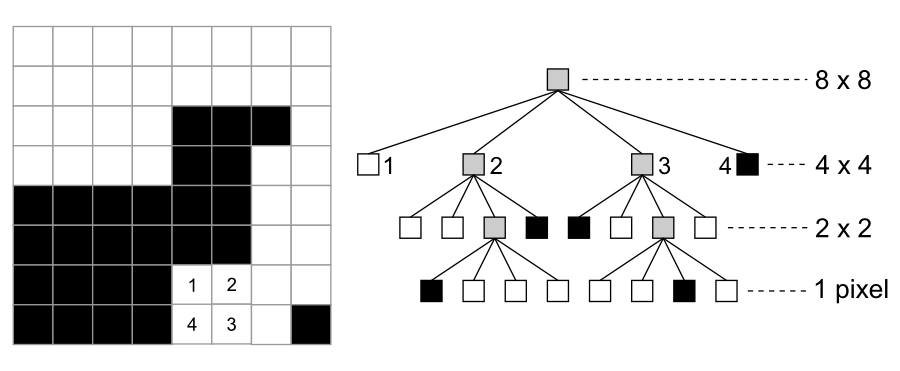
\includegraphics[scale=0.8]{images/quadtree.png}
	\caption{Représentation d'un quadtree.}
	\label{fig:quadtree}
\end{figure}

\begin{figure}[H]
	\centering
	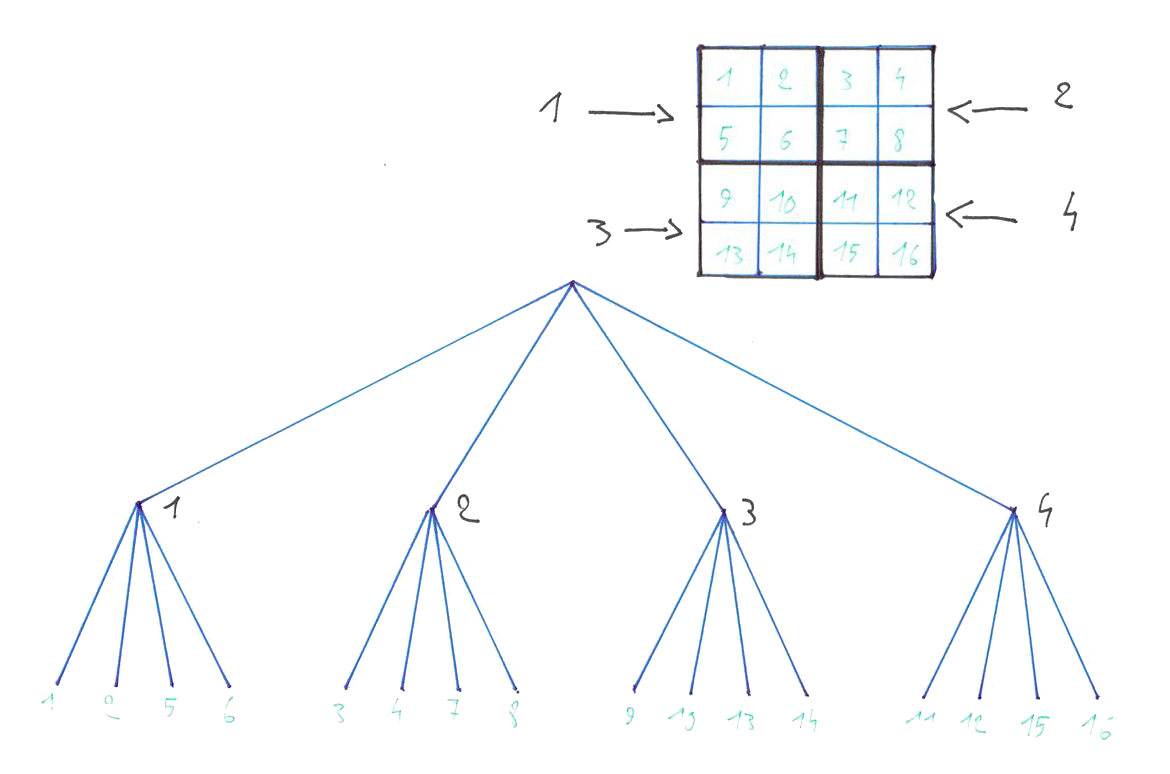
\includegraphics[scale=0.4]{images/quadtree-dessin.jpg}
	\caption{Représentation d'un quadtree.}
	\label{fig:quadtree2}
\end{figure}

Le passage d'un niveau $k$ au niveau $k + 1$ est représenté dans la figure \ref{fig:quadtree-niveaux}. Plus la valeur d'un niveau est élevée plus l'image est petite.

\begin{figure}[H]
	\centering
	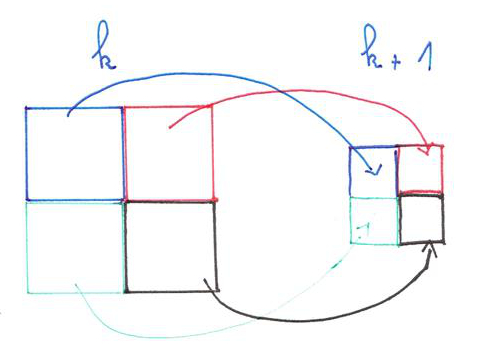
\includegraphics[scale=0.6]{images/quadtree-niveaux.jpg}
	\caption{Représentation du passage d'un niveau à un autre d'un quadtree.}
	\label{fig:quadtree-niveaux}
\end{figure}

	\chapter{L'algorithme}
		\section{Déroulement}
			L'algorithme détaillé dans l'article se déroule en 3 étapes. On applique tout d'abord un lissage par quadtree, puis une classification statistique des points sur le niveau le plus haut du quadtree. On termine enfin par une estimation des frontières.
		\section{Le lissage}
			La première étape de l'algorithme de segmentation d'image est un lissage effectué à l'aide d'un quadtree. Nous allons d'abord voir comment un quadtree peut être utilisé dans ce contexte puis comment le lissage est effectué.

\subsection{Utilisation d'un quadtree}
	Afin de former notre quadtree, nous allons commencer par créer le niveau $k = 0$ de l'arbre, c'est-à-dire les feuilles. Ce niveau va contenir tous les pixels de l'image, chaque valeur étant stockée dans un des nœuds. Puis on forme les niveaux supérieurs en faisant la moyenne des nœuds par groupe de 4. Chaque nœud n'étant pas une feuille a donc pour la valeur la moyenne de ses quatre fils. Chaque niveau de l'arbre donne donc une nouvelle image lissée.\\

	Prenons une image de taille $N \times N$, avec $N = 2^m$. On note $d(i,j)$ le pixel de coordonnées $(i,j)$ de l'image, avec  $0 \leq i \leq N$ et $0 \leq j \leq N$. On note $q(i,j,k)$ le nœud de l'arbre correspondant au pixel de coordonnée $(i,j)$ de l'image au niveau $k$ de l'arbre, avec $0 \leq i \leq 2^{m-k}$, $0 \leq j \leq 2^{m-k}$ et $0 \leq k \leq m$.\\

	Le rang $k = 0$ correspond simplement aux données, on a donc \[q(i,j,0) = d(i,j)\]

	Puis chaque nœud a pour valeur la moyenne de ses quatre fils, donc pour $k > 0$,
	\[ q(i,j,k) = \frac{q(2i, 2j, k-1) + q(2i+1, 2j, k-1) + q(2i, 2j+1, k-1) + q(2i+1, 2j+1, k-1)}{4}\]

	% petit schéma montrant quel nœud de l'arbre correspond à quel pixel et la réduction de la taille de l'image

	On remarque que plus k augmente et plus l'image est lisse (un pixel a pour valeur la moyenne de 4 autres) et est de petite taille. Il nous suffit dont de prendre un niveau suffisant de l'arbre pour avoir une image lisse. La question reste de déterminer le niveau optimal $m'$ pour lequel le lissage est suffisant sans pour autant que l'image soit trop dégradée pour effectuer les étapes suivantes de segmentation. Dans la partie suivant nous verrons comment déterminer ce niveau $m'$.

\subsection{Détermination du niveau optimal}
	Afin de trouver le niveau de lissage maximum $m'$ pour lequel on peut toujours effectuer la segmentation, on pose $r = 2^n$, le rayon minimal des régions que l'on souhaite détecter et qui doit être fixé a priori.

	En coupant le quadtree au niveau $m'$, on pourra détecter toutes les régions de rayon supérieur à $2^{m'+1}$. Pour détecter les régions de rayon $r=2^n$, on veut donc
	\[ 2^{m'+1} \leq 2^n \]
	\[ \Leftrightarrow m'+1 \leq n \]
	\[ \Leftrightarrow m' \leq n-1 \]

	On cherche à lisser notre image le plus possible tout en gardant une résolution suffisante pour détecter les régions de rayon $r$, on veut donc maximiser $m'$ tout en respectant $m' \leq n-1$, on a donc $m' = n-1$.
		\section{Classification statistique}
			\subsection{Algorithme du barycentre local}
	Une fois le niveau de lissage déterminé dans le quadtree, il faut classifier les différents pixels de l'image dans plusieurs régions. L'algorithme utilisé est celui du barycentre local (en anglais \textit{local centroid algorithm}). L'utilisation de cet algorithme ne requiert pas la connaissance du nombre de régions \textit{a priori}, contrairement par exemple à celui des K-moyennes (cf. partie \ref{subsubsec:segmentationClassification}). C'est un processus itératif qui se base sur l'histogramme de l'image et le niveau des gris des pixels environnants.\\

	L'algorithme peut-être défini à l'aide de cette procédure itérative :\\
	\[ h^n(i) = \sum_{j \in \Lambda^n(i)}^{} h^{n-1}(j) \mbox{ et } h^0(i) = h(i) \]
	\[\mbox{où } j \in \Lambda^n(i) \mbox{ si et seulement si } i = Ent[\frac{\sum\limits_{k=-m}^{m} kh( j + k)}{\sum\limits_{k=-m}^{m} h(j + k)}] \]

	Ces équations traduisent la recherche d'un centre de gravité dans une fenêtre de taille $2m + 1$.

\subsection{Convergence de l'algorithme}
	Il est difficile de démontrer théoriquement la convergence de l'algorithme, mais en pratique il a été observé que celui-ci converge rapidement, typiquement entre 10 et 20 itérations. Le nombre de classes dépend de la taille de la fenêtre et de l'importance des pics dans l'histogramme de l'image $h(i)$.

\subsection{Taille de fenêtre}
	La taille de la fenêtre est déterminée à l'aide d'un processus itératif. Cette taille est augmentée de 5 jusqu'à ce que plusieurs essais produisent des résultats similaires.

\subsection{Classification}
	La classification est effectuée une fois que l'algorithme du barycentre local a convergé. Pour chaque $i$, on cherche sa dernière valeur $i_n$ telle que $i_{k-1} \in \Lambda^k (i_k) \mbox{ avec } 1 \leq k \leq n \mbox{ et } i_0 = i$.
		\section{Estimation de la frontière}
			Cette partie de l'algorithme a pour but de redefinir les classes des pixels proches des frontières entre 2 régions afin de suprimer les noeuds isolés (ceux qui ont une classe différentes de ceux qui l'entourent), et ainsi de diminuer les erreurs. Cette partie s'organise en trois étapes : identification des noeuds appartenant à la frontière, leur lissage via l'application d'un filtre linéaire et la réafféctation des classes. Ces étapes sont effectuées sur chaque niveau du quadtree.

\subsection{Identification de la frontière}
	Nous allons tout d'abord chercher à identifier les noeuds situés sur la frontière entre deux régions. Pour cela nous allons travailler sur le niveau $m'$ du quadtree, sur lequel la classification a été effectuée, et sur l'image correspondante. 

	Un pixel appartient à la frontière $B(k)$ si un des ces huits voisins possède une classe différente de celle du pixel. Ainsi :

	\[ q(i,j,k) \in B(k) \Leftrightarrow c[q(i,j,k)] \ne c[q(i',j',k)] \]
	\[ (i',j') \in N_8(i,j) \]

	En appliquant ceci à chaque pixel de l'image nous avons determiné lesquels appartenaient à $B(k)$. Prenons par exemple une frontière en ligne droite définie selon (figure). B(k) sera alors défini selon la fiogure (figure)\\

	Nous allons maintenant chercher à determiner $B_1(k)$. L'union de $B(k)$ et de $B-1(k)$ nous donnera les pixels appartenant aux frontière.

	Un pixel appartient à $B_1(k)$ si un des ces huits voisins appartient à $B(k)$. Ainsi la frontière que nous avions définie précédemment "s'épaissit". Ainsi :

	\[ q(i,j,k) \in B_1(k) \Leftrightarrow q(i',j',k) \in B(k) \]
	\[ (i',j') \in N_8(i,j) \]

	et \[ B_c(k) = B(k) \cup B_1(k) \]

	Ainsi pour l'example précédent nous obtenons (figure).Nous allons maintenant travailler sur $B_c(k)$, que nous considérons comme notre frontière. 

\subsection{Lissage}
	Maintenant que nous connaissons les pixels appartenant à la frontière $B_c(k)$, nous allons les lisser grâce à une filtre linéaire. Nous allons maintenant définir le filtre linéaire utilisé.
	On note $\hat{\mu}_1$ et $\hat{\mu}_2$ les moyennes des deux classes que la frontière sépare et $\hat{\mu}(i,j,k)$ la moyenne de la classe associée au pixel $(i,j,k)$. 
	Soit $B_c'(k)$ l'ensemble des pixels n'appartenant pas à la frontière.

	On définit \[ \hat{\sigma}_k^2 = \frac{\sum\limits_{(i,j) \in B_c'(k)}[q(i,j,k)-\hat{\mu}(i,j,k)]^2}{N(B_c'(k))} \]

	$N(A)$ correspondant au nombre de points à l'intérieur de la région $A$.

	Soit \[ \hat{\rho}_k = \frac{\hat{\mu}_1 - \hat{\mu}_2}{\hat{\sigma}_k^2} \]

	Notre filtre linéaire est alors défini par 

	\[ h(\rho) = \left\lbrace\begin{array}{cc}
		\lambda(\rho) & \mbox{si } (i,j) = (0,0), \\
		\frac{1 - \lambda(\rho)}{8} & \mbox{sinon}\\
	\end{array}\right.
	\]

	$\lambda(\rho)$ étant une fonction linéaire par partie de $\rho$.

	On applique le filtre en effectuant une convolution : 
	\[ B_2(k) = h(i,j,\hat{\rho}_k) * B_c(k) \] 

\subsection{Réaffectation des classes}
	L'application du filtre nous a permis de lisser les pixels appartenant à la frontière. Nous allons maintenant réaffecter leurs classes à ces pixels en leur attribuant la classe dont la moyenne est la plus proche.

\subsection{Répétion aux autre niveaux}
	Les trois étapes précédentes sont répétées aux niveaux inférieurs du quad tree. On doit tout d'abord affecter les classes aux pixels en affectant aux fils la même classe que leur père. On applique ensuite à ce niveau l'identification de la frontière, le lissage et l'affection des classes. On répète l'opération au niveau inférieur et ainsi de suite jusqu'au niveau $k=0$, correspondant aux données initiales. 

	\chapter{Conclusion}
		Suite à l'analyse de cet article scientifique, nous sommes maintenant conscients des différentes techniques de segmentation qui existent et de leurs spécificités générales. En étudiant l'algorithme décrit dans cet article, nous avons vu comment l'utilisation des statistiques et des propriétés spatiales d'une image pouvaient permettre de définir plusieurs régions dans une image. Nous avons apprécié l'utilisation d'une structure de données originale, à savoir le quadtree, qui est l'élément sur lequel toutes les analyses sont effectuées.\\

Nous avons mis un certain temps à comprendre en détail toutes les parties de l'algorithme, en particulier les parties portant sur les estimations des erreurs, mais nous avons apprécié l'effort que nous avons effectué. Nous pensons pouvoir affirmer que nous connaissons maintenant les techniques de segmentation et que nous avons bien compris les différentes étapes de l'algorithme décrit dans l'article : lissage, classification statistique, estimation des frontières. Nous espérons avoir réussi à expliquer ces multiples étapes clairement dans ce rapport.

	%% -- Bibliographie
	\bibliographystyle{plain}
	\bibliography{bib}

\end{document}